\label{chap:06_contextualized_hate_speech}

En este capítulo analizamos el impacto de añadir contexto en la tarea de detección de discurso de odio en redes sociales. Como hemos marcado en los capítulos anteriores, la utilización del contexto ha recibido poca atención en la literatura, limitando la tarea a analizar comentarios aislados de cualquier tópico relacionado o hilo conversacional. Para este estudio, utilizamos el conjunto de datos construído en el Capítulo \ref{chap:05_dataset_creation}, cuyos datos constan de comentarios de artículos periodísticos en Twitter.

El formato de los datos empleados nos brinda información adicional a cada comentario tanto por el tweet del medio periodístico al que contestan como así también por el contenido del artículo. Para evaluar si la adición de contexto resulta en una mejora en la detección de discurso de odio, realizamos experimentos de clasificación con modelos que consumen tres tipos de entrada: el comentario sin contexto, el comentario junto al tweet del medio periodístico, y el comentario junto al tweet y el cuerpo del artículo asociado.

\todo{buscar todos los verbos conjugados en futuro}

El conjunto de datos empleado nos permite analizar una posible combinación más en base al detalle de las características ofendidas por cada comentario. Esta información granular permite no sólo analizar la existencia de discurso de odio sino que permite predecir con más detalle la ofensa cometida. Proponemos en base a esto dos tareas de clasificación: una tarea de detección \textbf{binaria}, donde sólo predecimos si hay o no discurso de odio; y una tarea de detección \textbf{granular}, donde además predecimos todas las características ofendidas (potencialmente más de una). Para estas tareas, propusimos algoritmos de clasificación sobre modelos pre-entrenados de lenguaje que tienen como entrada los distintos tipos de contexto posibles. Estos modelos tienen incorporados naturalmente la posibilidad de consumir dos entradas --el contexto y el texto-- con lo cual son ideales para nuestros experimentos.

Evaluamos los resultados de los experimentos de clasificación tanto en términos del rendimiento de las distintas configuraciones de nuestros clasificadores, como así también realizando análisis de error comparativos entre los modelos contextualizados y los no contextualizados. También evaluamos en este capítulo las dificultades más generales que presenta la detección de este fenómeno sobre comentarios de notas periodísticas.

\section{Trabajo previo}
\label{sec:06_classification_previous}

Como mencionamos en la Sección \ref{sec:dataset_previous}, no se ha dado demasiada atención en la literatura a la utilización de información contextual en la detección de discurso de odio y otros fenómenos similares. Pasamos ahora a repasar los algoritmos de detección utilizados sobre los conjuntos de datos descriptos en dicha sección.

\citet{gao-huang-2017-detecting} proponen utilizar dos tipos de modelos sobre el dataset que ellos mismos recolectaron sobre comentarios de Fox News: regresiones logísticas y redes neuronales recurrentes. Para las regresiones logísticas, usaron como entradas bolsas de palabras, bolsas de caracteres, vectores semánticos producidos con Linguistic Inquiry and Word Count (LIWC) \cite{pennebaker2001linguistic}, y otras variables de un lexicón de emociones \cite{mohammad2013nrc}. Por otro lado, los autores también entrenan LSTM bidireccionales con mecanismo de atención de Bahdanau \cite{bahdanau2014neural} que consumen embeddings \emph{word2vec} de dimensión 100.

Un punto criticable de este trabajo es que utiliza el nombre de usuario como entrada, algo que a priori no suele hacerse ya que permitiría prejuzgar a un usuario antes que por el contenido de sus tweets. Si bien es cierto que la información de usuarios y sus conexiones es valiosa, introducir esta información a nuestros modelos puede dar lugar a correlaciones espurias que es preferible evitar. Otras críticas sobre el proceso de anotación de los datos fueron realizadas ya en la Sección \ref{sec:dataset_previous}.


\begin{figure*}[t]
    \centering
    \begin{minipage}[b]{0.49\textwidth}
        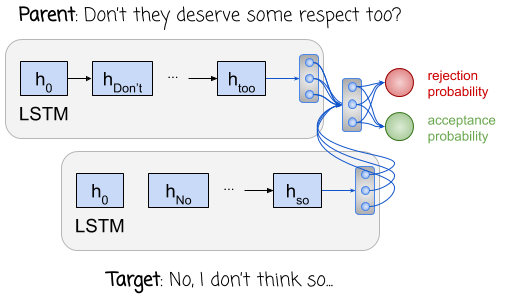
\includegraphics[width=\textwidth]{img/pavlopoulos_rnn_rnn_classifier.png}
    \end{minipage}
    \hfill
    \begin{minipage}[b]{0.49\textwidth}
        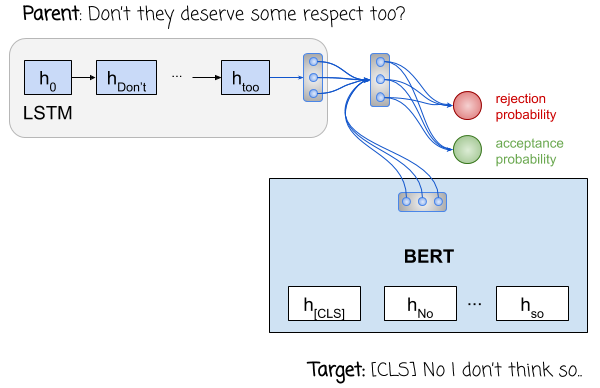
\includegraphics[width=\textwidth]{img/pavlopoulos_rnn_bert_classifier.png}
    \end{minipage}

    \begin{minipage}[b]{0.35\textwidth}
        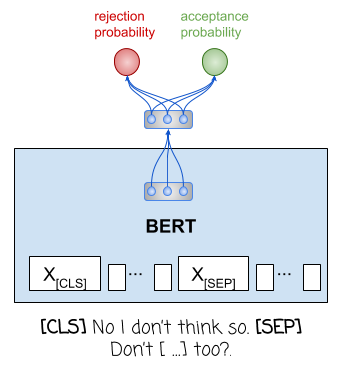
\includegraphics[width=\textwidth]{img/pavlopoulos_bert_sep_classifier.png}
    \end{minipage}


    \caption{Clasificadores que consumen contexto propuestos por \citet{pavlopoulos2020toxicity}. Los dos primeros clasificadores proponen una arquitectura de dos encoders, uno para el texto y otro para el contexto usando bi-LSTMs y BERT como posibilidades. El tercer clasificador propuesto es un BERT usando su estructura natural para codificar dos oraciones separadas por el token $SEP$ }
    \label{fig:pavlopoulos_classifiers}
\end{figure*}


En la Sección \ref{sec:dataset_previous} hemos descripto el conjunto de datos construído por \citet{pavlopoulos2020toxicity}, dedicado a la detección de toxicidad y que incorpora información conversacional sobre comentarios de Wikipedia Talk Pages. Nos detenemos un momento para analizar sus experimentos de clasificación ya que guardan importantes similaridades con lo hecho en este capítulo. En ese trabajo se obtuvieron dos conjuntos de entrenamiento: uno en el cual los etiquetadores tenían información del contexto, y otro conjunto en el que no. El conjunto de test, por otro lado, fue anotado teniendo en cuenta el contexto bajo la asunción de que el etiquetado es de mejor calidad al tener más información contextual. Sobre la base de estos datos, los autores plantearon dos preguntas:

\begin{itemize}
    \item ¿Mejora el rendimiento de los clasificadores que son entrenados con el conjunto de datos etiquetado con contexto?
    \item ¿Mejora el rendimiento de los clasificadores consumiendo información contextual?
\end{itemize}

Para responder estas preguntas, los autores consideraron las siguientes combinaciones para sus experimentos: utilizar conjunto de entrenamiento etiquetado con o sin contexto, y entrenar el clasificador con o sin contexto. Para aquellos clasificadores que no consumen contexto, los autores consideraron las mismas alternativas que hemos visto en capítulos anteriores: bi-LSTM o \bert{}. Para aquellos que sí consumen contexto, se evaluaron dos estrategias: la primera consistió en usar una única red que codifique la entrada del texto y el contexto concatenada con un token especial; la segunda consistió en usar dos codificadores distintos para el contexto y el texto. Para la segunda alternativa, y dados los recursos computacionales disponibles, no utilizaron dos modelos pre-entrenados, sino un codificador LSTM para el contexto y un \bert{} para el texto. A su vez, también utilizaron la API Perspective de Google con la misma estrategia de concatenación. Para todas las combinaciones posibles, la mejora en el rendimiento resultante de disponer de información contextual no es estadísticamente significativa.

Dos versiones de \bert{} fueron utilizadas como base para entrenar los modelos de Transformers: una, usando los pesos del modelo de \bert{} de \citet{devlin2018bert}; y la segunda, haciendo un ajuste de dominio de \bert{} sobre un dataset grande y no etiquetado relacionado a la tarea en cuestión. Este proceso de \emph{ajuste de dominio} o \emph{fine-tuning} consiste en ajustar el modelo de lenguaje sobre un conjunto de datos no etiquetados y afines a nuestra tarea final. Esta técnica ha demostrado ser efectiva para lograr mejoras sensibles en el desempeño de clasificadores sobre dominios particulares \cite{gururangan-etal-2020-dont}, y será estudiada más detenidamente en el Capítulo \ref{chap:07_domain_adaptation}. Para este trabajo, el ajuste es realizado sobre un subconjunto de comentarios del dataset de \emph{Civil Comments} \cite{borkan2019civil} sin ningún tipo de contexto. A priori, ajustar el modelo de lenguaje sobre comentarios a secas podría inducir a pensar que puede deteriorar el rendimiento al entrenar posteriormente sobre contexto; sin embargo, en la versión no adaptada de \bert{} tampoco se observó una mejora significativa en el rendimiento.

Algunas limitaciones de este trabajo marcadas por los autores son:

\begin{itemize}
    \item Contexto muy pequeño: sólo se consideraron como contexto el título de la discusión de Wikipedia Talk Pages y adicionalmente el comentario previo.
    \item El hilo completo de los comentarios es ignorado: sólo se observa el comentario previo.
    \item Los comentarios fueron muestreados aleatoriamente, sin tener en cuenta algunos ámbitos más propicios para la toxicidad.
\end{itemize}

\citet{xenos-2021-context} continuaron el trabajo de \citet{pavlopoulos2020toxicity} reetiquetando el conjunto de datos de Civil Comments con información contextual y --como mencionamos en la Sección \ref{sec:dataset_previous}-- presentando una nueva tarea de detección de sensibilidad al contexto. Usando la API Perspective (y la estrategia de concatenación básica de texto y contexto) notaron que la performance del clasificador contextualizado mejora sensiblemente si restringimos nuestra atención a comentarios más sensibles a su entorno de acuerdo a la métrica definida. De esto último puede concluirse que, a diferencia del trabajo anterior, si bien  el contexto no es realmente necesario para comprender la toxicidad del grueso de los comentarios, hay cierto subconjunto para los cuales esta información adicional resulta relevante.


\section{Tareas de clasificación propuestas}
\label{sec:tasks}

Para analizar el impacto del contexto en la detección de discurso de odio, y teniendo en cuenta que contamos de un dataset con anotaciones granulares sobre las características ofendidas, propusimos dos tareas de clasificación:

\begin{enumerate}
    \item \textbf{Detección binaria}: Dado un tweet y su contexto, predecir si es discriminatorio.
    \item \textbf{Detección granular}: Dado un tweet y su contexto, predecir las características ofendidas (de haber alguna) y si contiene un llamado a la acción.
\end{enumerate}

%%
%%
%% Link
%% https://docs.google.com/drawings/d/11sAaOuGJlU0P61mkrPxKduFwnNOuPV31tXUFJWEwbVU/edit?usp=drive_web&ouid=117313784631536396179
%%
%%
\begin{figure}[t]
    \centering
    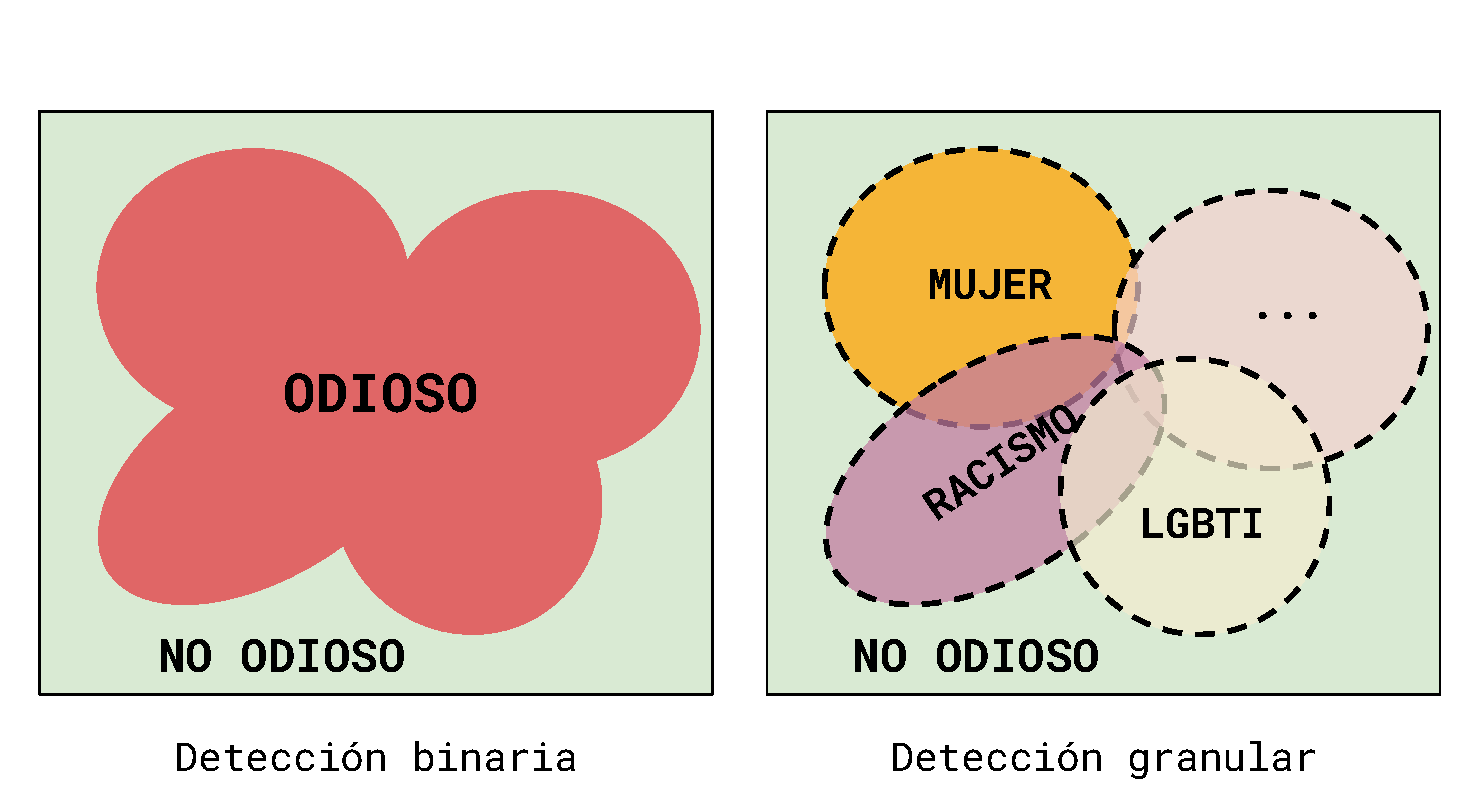
\includegraphics[width=\textwidth]{img/06/hate_detection_tasks.pdf}
    \caption{Tareas propuestas de detección de discurso de odio. La tarea de detección binaria consta de predecir si un tweet contiene contenido discriminatorio, discriminando la frontera conjunta de todas las características. En la tarea granular, predecimos por separado cada una de las características ofendidas, pudiendo haber más de una o bien ninguna.}
    \label{fig:hate_detection_tasks}
\end{figure}



Puede pensarse la tarea de detección binaria (la que usualmente se aborda en la literatura sobre el tema) como una relajación de la tarea granular: mientras la primera sólo nos permite detectar si hay o no contenido discriminatorio, la segunda requiere información más precisa acerca de las características ofendidas, permitiendo a su vez tener mayor información sobre la salida de los clasificadores y dando lugar a una mejor interpretación de sus errores. La Figura \ref{fig:hate_detection_tasks} ilustra las dos tareas propuestas en forma de Diagrama de Venn: mientras en la tarea binaria sólo debemos decidir de qué lado de la frontera se encuentra un comentario (si tiene o no discurso de odio) en la tarea granular se debe decidir esto mismo para cada una de las características,


Viendo las tareas propuestas como problemas de clasificación, la detección binaria consta de predecir una sola etiqueta binaria, mientras que la tarea granular consta de predecir $n$ etiquetas binarias. Esto último puede también verse como $n$ problemas distintos de clasificación, o una tarea de \tbf{multiclasificación}. Una observación sobre estos dos enfoques del problema es que podemos construir un clasificador para la tarea binaria a través de un clasificador entrenado para la tarea granular tomando la disyunción lógica de sus salidas: hay discurso de odio sí y sólo sí hay al menos una característica ofendida. Retomamos esta idea más adelante al hablar de cómo evaluamos nuestras técnicas de clasificación para cada tarea.


\begin{table}[h]
    \centering
    \begin{tabular}{l c r}
        \toprule
        Partición     & Artículos       &  Comentarios         \\
        \midrule
        Entrenamiento & \mr{2}{990}     & \num{36420}                    \\
        Desarrollo    &                 & \num{9106}                    \\
        \hline
        Test          & \num{248}       & \num{11343}           \\
        \bottomrule
    \end{tabular}
    \caption{Particiones del conjunto de datos utilizado para las dos tareas}
    \label{tab:data_splits}
\end{table}

Para las dos tareas utilizamos el conjunto de datos construido en el Capítulo \ref{chap:05_dataset_creation} separando las instancias en tres particiones: entrenamiento, desarrollo, y test. Para las dos primeras (entrenamiento y desarrollo) reservamos \num{990} artículos mientras que  para el dataset de test tomamos \num{248} artículos y sus comentarios. Ambos conjuntos de noticias son disjuntos para intentar maximizar las instancias realmente diferentes para las etapas de entrenamiento y evaluación. Sobre los primeros \num{990} artículos, dividimos el conjunto en \num{36420} instancias de entrenamiento y \num{9106} instancias de desarrollo, sin garantizar que provengan de notas periodísticas distintas.


\section{Modelos de clasificación}
\label{sec:contextualized_classifiers}


Entrenamos clasificadores neuronales basados en el modelo pre-entrenado \beto{} \cite{canete2020spanish} tanto para la tarea binaria como para la granular. Incorporamos la información contextual en cada comentario teniendo en cuenta tres tipos de entrada por instancia: el comentario sin ningún tipo de contexto (notaremos \tbf{sin contexto}), el comentario con el tweet al que responde como contexto (\tbf{tweet}), y finalmente el comentario con el tweet al que responde y el texto del artículo periodístico (\tbf{tweet + artículo}). Para las dos versiones que consumen información contextual, separamos el texto y el contexto con el token especial \septok{}.

%%
%%
%% Link a Draw
%% https://docs.google.com/drawings/d/1F8iVSIRqHhGkQ0zglxqXLGD36RHZ9OhHMZYsg_xFOS4/edit
%%
%%

\begin{figure}
    \centering
    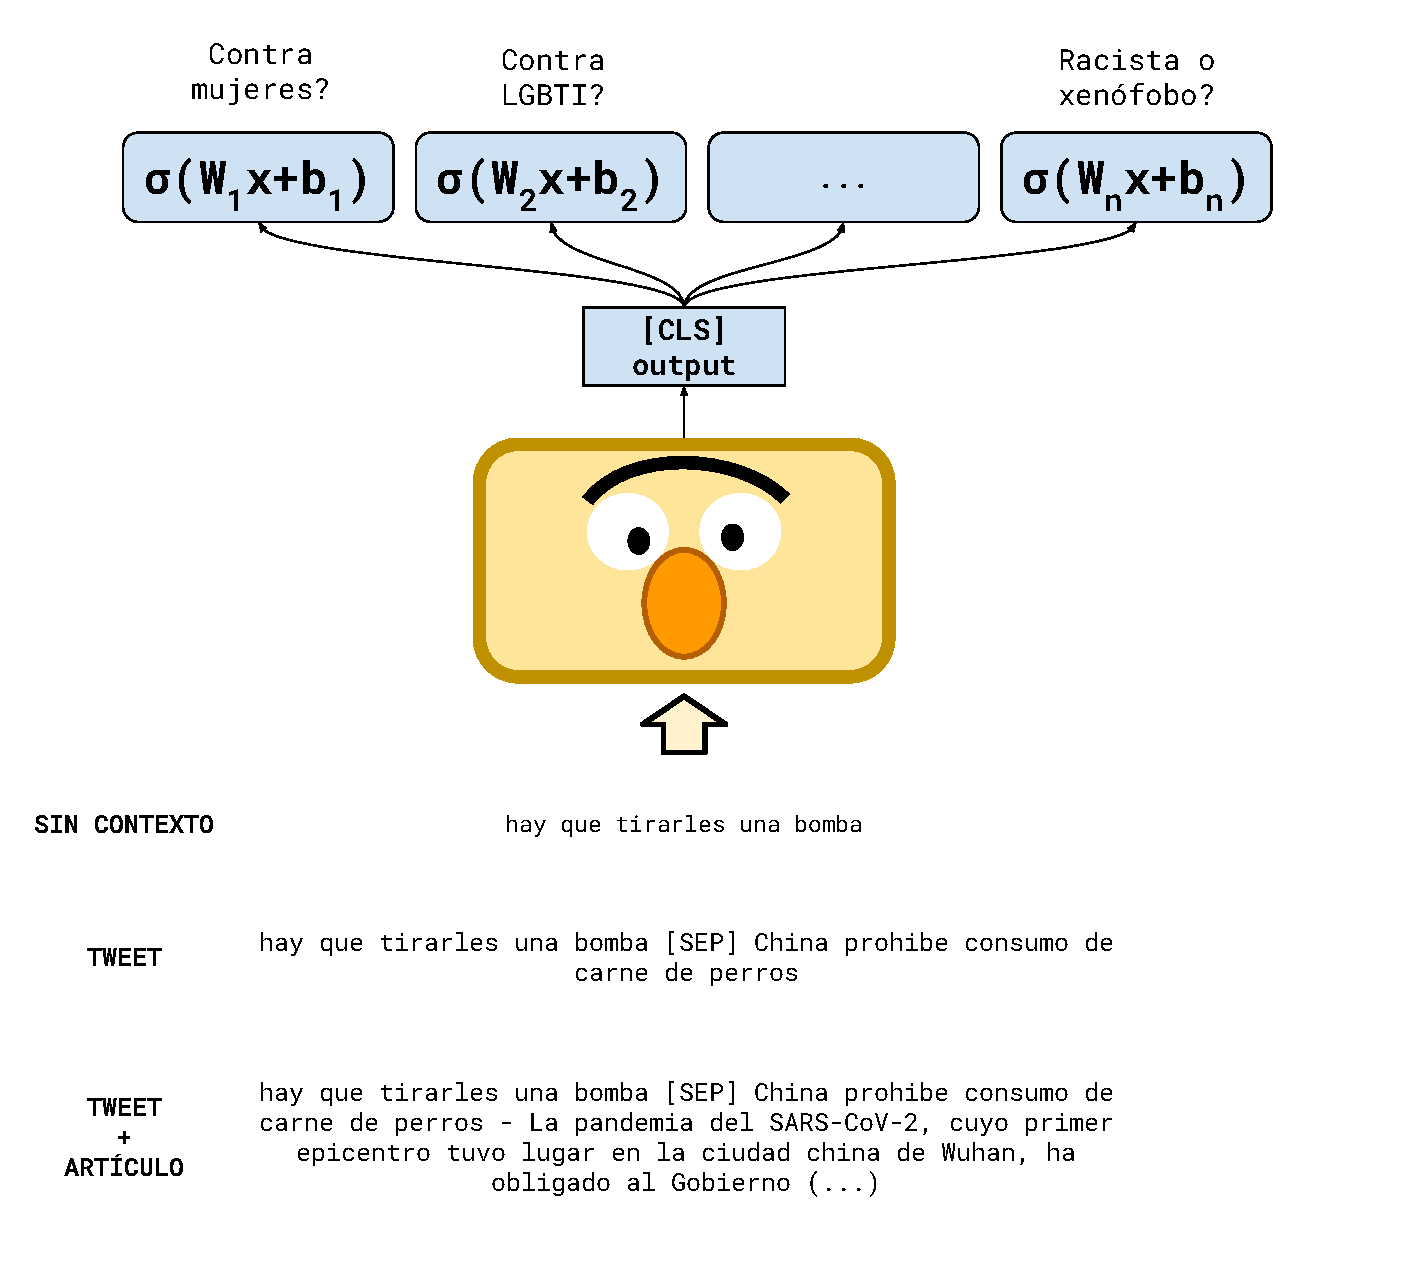
\includegraphics[width=1.10\textwidth]{img/06/bert_contextual_classifier.pdf}
    \caption{Modelo de multiclasificación para la tarea granular basado en \beto{}. Los modelos son entrenados de tres maneras distintas: sin contexto (sólo el comentario), con el contexto del tweet, y con el contexto del tweet y el texto del artículo. La salida consta de la probabilidad de que el comentario tenga contenido odioso para alguna de las características en cuestión o bien contenga una llamada a la acción}
    \label{fig:05_multi_bert_classifier}
\end{figure}

Para la tarea binaria, la salida es la estándar para un clasificador binario. En cuanto a la tarea de detección granular, la abordamos de manera similar a la \subtaskb{} del Capítulo \ref{chap:04_hate_speech}, en este caso como la predicción de nueve variables distintas: llamado a la acción (CALLS) y las ocho características ofendidas (MUJER, RACISMO, CLASE, LGBTI, CRIMINAL, ASPECTO, DISCAPACIDAD, POLITICA). En lugar de entrenar un clasificador diferente por cada característica, entrenamos un modelo de multiclasificación BERT que comparte todos sus pesos salvo nueve capas lineales de salida distintas.

Como función de costo, empleamos la suma de las funciones de costo de cada característica. Concretamente, si $y$ son las etiquetas de un comentario e $\widehat{y}$ las predicciones del modelo:

\begin{equation*}
    L(y, \widehat{y}) = \sum\limits_{\mathclap{c \in CHAR'}} J(y_c, \widehat{y}_c)
\end{equation*}

\noindent donde $CHAR'$ es el conjunto de todas las características protegidas junto a la variable de llamada a la acción (CALLS), y $ J$ es la función de entropía cruzada. Compartir los pesos entre todas las salidas tiene dos objetivos: primero, poder generar un modelo más compacto (de otra forma serían nueve BERT distintos que suman alrededor de \num{1000}M parámetros) y segundo, compartir información común entre las distintas características atacadas, ya que guardan similaridades y muchas de ellas tienen una importante intersección, como hemos visto en la Sección \ref{sec:analisis_dataset_por_caracteristica}.

Para tener costos computacionales más amigables, limitamos los largos de las secuencias a 128, 256 y 512 tokens para los modelos con entrada sin contexto, tweet, y tweet+cuerpo respectivamente. Preprocesamos ambos tweets --contexto y texto-- utilizando las técnicas descriptas en la Sección \ref{sec:03_preprocessing}: conversión de usernames a un token especial (\verb|usuario|), tratamiento de hashtags (separación e inserción de un hashtag especial), y conversión de emojis a su representación textual. La Figura \ref{fig:05_multi_bert_classifier} ilustra el modelo de clasificación para la tarea granular, junto a los tres tipos de entrada considerados. La configuración de hiperparámetros utilizados en el entrenamiento es la misma que la detallada en la Sección \ref{sec:03_classification}.

\subsection{Adaptación de dominio}

Una práctica cada vez más extendida en trabajos del área de clasificación de documentos es realizar una adaptación de dominio para mejorar la performance sobre la tarea final. La técnica de adaptación de dominio para modelos de lenguaje pre-entrenados consiste en continuar el pre-entrenamiento sobre un dataset grande y no supervisado relacionado a nuestro dominio o directamente sobre el dataset de la tarea si no tenemos acceso a otros datos \cite{gururangan-etal-2020-dont}. En la Sección \ref{sec:domain_adaptation_previous_work} del siguiente capítulo haremos una reseña más extensa de esta técnica, pero por lo pronto podemos entender que esta técnica ajusta el modelo de lenguaje a nuestros datos, ya que estos pueden tener diferencias considerables respecto de los empleados en el pre-entrenamiento. En nuestro caso puntual, mientras \beto{} fue entrenado en Wikipedia y textos formales, nuestro dominio consta de comentarios en Twitter a notas periodísticas, con expresiones muy distintas a las encontradas en medios más formales.

\begin{table}[t]
    \centering
    \begin{tabular}{lr}
        \toprule
        Hiperparámetro & Valor         \\
        \midrule
        Pasos               & \num{10000}           \\
        Tamaño de batch     & \num{2048}            \\
        Tamaño de secuencia & 128, 256 y 512  \\
        $\beta_1$           & $0.9$           \\
        $\beta_2$           & $0.98$          \\
        $\epsilon$          & $10^{-6}$       \\
        Decay               & $0.01$          \\
        LR pico             & $0.0004$     \\
        Pasos de warmup     & $0.1$             \\
        \bottomrule
    \end{tabular}
    \caption{Hiperparámetros para la adaptación de dominio de BERT}
    \label{tab:hs_ft_hyperparameter}
\end{table}


\citet{pavlopoulos2020toxicity} realizaron una adaptación de dominio sobre los comentarios del corpus de \emph{Civil Comments} sin utilizar ningún tipo de contexto. Proponemos, a diferencia de este trabajo, tres tipos de adaptaciones de acuerdo al contexto considerado: una adaptación sin contexto, una adaptación con el contexto del tweet, y una adaptación con el contexto del tweet y el cuerpo de la noticia. Los datos usados para este ajuste fueron el sobrante de la recolección del anterior capítulo: alrededor de $288$ mil artículos con $5$ millones de comentarios que no están incluídos en el conjunto de datos etiquetado \footnote{Utilizamos algunos datos extra recolectados a posteriori de lo mencionado en el capítulo anterior}.



\citet{liu2019roberta} recomienda descartar en el pre-entrenamiento de modelos de lenguajes el objetivo NSP, con lo cual realizamos nuestro ajuste de dominio exclusivamente con la tarea de modelado de lenguaje enmascarado (MLM). La Tabla \ref{tab:hs_ft_hyperparameter} contiene los hiperparámetros utilizados al correr la adaptación de dominio correspondientes al optimizador Adam con warmup lineal para el learning rate. Estos ajustes los realizamos sobre una \emph{TPU v2-8} y una máquina de \emph{Google Colab Pro}, tomando alrededor de 10 hs en su largo de cadena máximo.

\subsection{Rendimiento humano en la tarea}


\begin{table}
    \centering
    \begin{tabular}{l cc  cc}
                   & \multicolumn{2}{c}{Entre anotadores} & \multicolumn{2}{c}{Contra etiquetas} \\
        {}         &  F1 media &  F1 mediana  & F1 media  &  F1 mediana \\
        \hline
        ODIO       &  $65.3$ &   $67.5$    & $82.9$   &   $85.1$   \\
        CALLS      &  $43.4$ &   $49.5$   &  $70.4$   &   $84.2$  \\
        \hline
        MUJER      &  $49.0$ &   $46.8$   &  $74.1$   &   $75.9$  \\
        LGBTI      &  $59.6$ &   $57.7$   &  $84.6$   &   $91.5$  \\
        RACISMO    &  $65.3$ &   $64.4$   &  $87.1$   &   $87.9$  \\
        CLASE      &  $44.3$ &   $44.4$   &  $72.2$   &   $73.2$  \\
        POLITICA   &  $46.1$ &   $43.6$   &  $79.5$   &   $81.5$  \\
        DISCAPACIDAD& $55.0$ &   $60.0$   &  $81.3$   &   $84.2$  \\
        APARIENCIA &  $64.9$ &   $74.3$   &  $83.1$   &   $91.5$  \\
        CRIMINAL   &  $52.7$ &   $58.0$   &  $84.1$   &   $92.9$  \\
        \hline
        Macro F1   &  $53.4$ &   $55.4$   &  $79.6$   &   $84.8$  \\
        \hline
    \end{tabular}

    \caption{Estadísticos del F1 (en porcentaje) entre anotadores. Las dos primeras columnas marcan las métricas medidas entre anotadores, y las dos últimas la de los anotadores contra las etiquetas asignadas en el conjunto de datos. La Macro F1 es el promedio de los F1 todas las características y de la llamada a la acción (CALLS). }
    \label{tab:ia_f1_scores}
\end{table}

\todo{Cambiar ese CALLS en todos lados por favor}


La tarea de detección de lenguaje discriminatorio contiene una alta cantidad de ruido y un bajo acuerdo entre humanos, como se atestigua en recientes revisiones de los conjuntos de datos generados para su clasificación \cite{poletto2021resources}. En este escenario, cabe preguntarse una cota al rendimiento que puede lograr un algoritmo de detección automática para esta tarea, algo que esperamos --por la misma naturaleza del problema-- que diste mucho de la perfección. Si bien en muchos trabajos se ha logrado que algoritmos basados en Transformers superen el rendimiento humano para distintas tareas de NLP \footnote{Algo discutible dado que el rendimiento humano para estos benchmarks --como GLUE-- está medido a través de trabajadores contratados a través de crowdsourcing con pagas por debajo del salario mínimo}, consideramos el desempeño de nuestros anotadores como una cota superior razonable para las técnicas automáticas que hemos propuesto.

Para obtener números indicativos del rendimiento humano en la detección de discurso de odio, utilizamos la información recolectada durante la anotación del conjunto de datos. Consideramos las anotaciones de cada uno de los seis participantes en el proceso como predicciones y las evaluamos de dos formas: la primera tomando como etiquetas doradas las anotaciones de otro anotador; la segunda, tomando las etiquetas generadas en la Sección \ref{sec:asignacion}. En el primer caso tenemos $\binom{6}{2}=15$ combinaciones, mientras que en la segunda tenemos una para cada anotador, 6 combinaciones. Para estas dos formas de calcular rendimientos humanos, calculamos la medida \emph{F1} entre las predicciones de cada anotador y las etiquetas doradas, y calculamos medias y medianas para obtener estimaciones puntuales de los rendimientos.

Algo a tener en cuenta en la comparación contra las etiquetas del conjunto de datos es que este \emph{gold standard} es construido mediante votación mayoritaria de los dos o tres anotadores empleados, por lo cual estamos calculando la métrica entre dos variables correlacionadas. Mientras esta cota por un lado es muy grosera, por el otro, las métricas calculadas entre anotadores pueden ser algo bajas debido a que son predicciones muy ruidosas a diferencia de las etiquetas doradas que son más robustas al estar generadas por varios usuarios. El mejor escenario para estimar el rendimiento hubiera sido contar con una anotación extra para cada instancia y compararla contra la etiqueta dorada, aunque esta metodología es poco eficiente en términos de recursos.

La Tabla \ref{tab:ia_f1_scores} contiene las medias y medianas del puntaje F1 tanto entre anotadores como contra el \emph{gold-standard}. La mediana entre anotadores de la F1 es $67.5$, un puntaje relativamente bajo para la detección de odio, mientras que contra el gold standard es de $85.1$ puntos de F1; podemos suponer que la performance humana para la tarea se encuentra en algún lugar entre esos dos números. Respecto a las características, el rendimiento para su reconocimiento entre humanos en algunas de ellas se mantiene muy bajo, particularmente en MUJER, CLASE y POLITICA. Esto se desprende de las observaciones y dificultades descriptas en el Capítulo \ref{chap:05_dataset_creation} durante el proceso de anotación, como así también del hecho que estas características tienen un solapamiento no menor entre sí.



\section{Resultados}



\begin{table*}
    \centering
    \large
    \begin{tabular}{l P{0.08\textwidth}P{0.08\textwidth} P{0.08\textwidth}P{0.08\textwidth}  P{0.08\textwidth}P{0.08\textwidth}}
        \mr{2}{Métrica}          &\multicolumn{2}{c}{Sin Contexto}& \multicolumn{2}{c}{Tweet}          &  \multicolumn{2}{c}{Tweet + Cuerpo}    \\
                  & $\neg$FT &  FT     & $\neg$FT&    FT       &$\neg$FT &    FT \\
        \hline
        Accuracy  & $88.9$   &  $89.9$ & $90.2$  &$\mbf{91.0}$ & $90.4$  &  $90.5$ \\
        Precisión & $67.8$   &  $71.8$ & $73.1$  &$\mbf{74.8}$ & $73.9$  &  $72.8$ \\
        Recall    & $56.8$   &  $60.2$ & $60.1$  &$\mbf{65.3}$ & $61.1$  &  $64.1$ \\
        F1        & $61.8$   &  $65.5$ & $66.0$  &$\mbf{69.7}$ & $66.9$  &  $68.1$ \\
        Macro  F1 & $77.6$   &  $79.8$ & $80.1$  &$\mbf{82.2}$ & $80.6$  &  $81.3$ \\
        \hline
    \end{tabular}


    \caption{Resultados de los experimentos de clasificación para la tarea \emph{binaria} de detección de discurso de odio, expresados como la media de las distintas métricas sobre diez corridas independientes. En negrita, los mejores resultados. Cada modelo es un BERT con tres posibles entradas: sólo el comentario (\emph{Sin contexto}), el tweet de la noticia a la cual responde el comentario (\emph{Tweet}), y el tweet más el cuerpo de la noticia (\emph{Tweet + Cuerpo}). Para cada una de estas posibilidades usamos dos versiones: una sobre BETO ($\neg$FT) y otra sobre BETO ajustado al dominio (FT).}
    \label{tab:task_a_results}
\end{table*}


La Tabla \ref{tab:task_a_results} contiene los resultados para la tarea de clasificación \tbf{binaria} medidos por Accuracy, Precision, Recall, F1 de la clase positiva y Macro F1 entre las dos clases. Las métricas están expresadas como las medias de diez corridas independientes de los experimentos. Las seis columnas corresponden a la combinación de los tres posibles modelos dependiendo del contexto utilizado y de acuerdo a si ajustamos al dominio o no. Podemos observar que, en todos los casos, la adaptación de dominio (las columnas marcadas con FT) obtienen mejor rendimiento que los modelos que no están adaptados ($\neg$FT) resultando en una mejora de alrededor de 4 puntos de F1 en los casos sin contexto y con contexto de tweet. Entre los modelos sin ajustar a dominio, el que consume el contexto completo (tweet + cuerpo de la noticia) obtiene el mejor desempeño; sin embargo, esto no se replica en el caso ajustado a dominio, donde gana el contexto simple. Viendo sólo las columnas marcadas como $FT$, la mejora contra el modelo que no consume contexto es de $4.2$ puntos de F1. El modelo con el contexto completo, si bien mejora la performance general contra no tener contexto, pierde precisión al ser adaptado al dominio.


\begin{table*}
    \centering
    \Large
    \begin{tabular}{l P{0.08\textwidth}P{0.08\textwidth} P{0.08\textwidth}P{0.08\textwidth}  P{0.08\textwidth}P{0.08\textwidth}}
        Métrica        &\mc{2}{Sin Contexto}& \mc{2}{Tweet}          &  \mc{2}{Tweet + Cuerpo}    \\
                       & $\neg$FT&    FT    & $\neg$FT   &    FT     & $\neg$ FT&    FT     \\
        \hline
        LLAMA          & $64.6$ &    $65.1$   & $63.8$ &$\mbf{68.5}$  & $65.3$ &    $68.0$    \\
        MUJER          & $37.3$ &    $38.9$   & $41.1$ &$\mbf{42.1}$  & $38.1$ &$\mbf{42.1}$ \\
        LGBTI          & $35.1$ &    $36.6$   & $45.1$ &$\mbf{48.2}$  & $42.7$ &    $44.5$    \\
        RACISMO        & $63.5$ &    $65.3$   & $68.8$ &$\mbf{72.0}$  & $69.1$ &    $71.1$    \\
        CLASE          & $40.1$ &    $43.3$   & $49.1$ &$\mbf{51.1}$  & $45.1$ &    $47.6$    \\
        POLITICA       & $55.5$ &    $61.1$   & $57.9$ &$62.5$        & $59.1$ &$\mbf{64.8}$ \\
        DISCAPAC       & $55.1$ &    $58.2$   & $58.5$ &$\mbf{60.9}$  & $55.7$ &    $57.8$    \\
        APARIENCIA     & $72.6$ &    $74.2$   & $74.1$ &$\mbf{76.6}$  & $75.5$ &    $75.8$    \\
        CRIMINAL       & $51.3$ &    $52.9$   & $65.0$ &$\mbf{69.9}$  & $65.4$ &    $66.8$    \\
        \hline
        Macro F1       & $52.8$ &    $55.1$   & $58.2$ &$\mbf{0.613}$ & $57.3$ &    $59.8$    \\
        Macro Precision& $55.8$ &    $63.0$   & $64.2$ &$\mbf{0.702}$ & $67.7$ &    $67.8$    \\
        Macro Recall   & $50.6$ &    $49.9$   & $54.0$ &$\mbf{0.551}$ & $50.4$ &    $54.1$    \\
        % \hline
        % Hate Precision & 0.679 &    0.712   & 0.722 &\textbf{0.760}  & 0.748 &    0.741    \\
        % Hate Recall    & 0.621 &    0.631   & 0.642 &\textbf{0.666}  & 0.621 &    0.658    \\
        % Hate F1        & 0.648 &    0.668   & 0.679 &\textbf{0.710}  & 0.679 &    0.697    \\
        \bottomrule
        \end{tabular}
    \caption{Resultados de los experimentos de clasificación para la tarea \emph{granular} de detección de discurso de odio, expresados como la media de las distintas métricas sobre diez corridas independientes. Cada modelo es un BERT con tres posibles entradas: sólo el comentario (\emph{Sin contexto}), el tweet de la noticia a la cual responde el comentario (\emph{Tweet}), y el tweet más el cuerpo de la noticia (\emph{Tweet + Cuerpo}). Para cada una de estas posibilidades usamos dos versiones: una sobre BETO($\neg$FT) y otra sobre BETO ajustado al dominio (FT) de acuerdo a lo descripto en la Sección \ref{sec:contextualized_classifiers}}
    \label{tab:task_b_results}
\end{table*}



La Tabla \ref{tab:task_b_results} muestra los resultados de los experimentos de clasificación para la tarea de detección \tbf{granular} medidos en puntos de F1 para cada una de las características, y las métricas promediadas de precision, recall, y F1. Como era esperable, la ganancia de tener contexto disponible es más evidente en esta tarea, observándose una diferencia de aproximadamente 6 puntos de F1 entre la mejor versión sin contexto y la mejor versión con contexto ($55.1$ Macro F1 de la versión $FT$ sin contexto vs $61.3$ F1 de la versión $FT$ con el contexto del tweet). Respecto a los dos tipos de contexto, de nuevo la versión simple obtiene mejor rendimiento en prácticamente todas las características, con la única excepción de POLITICA.


\begin{figure*}[]
    \centering
    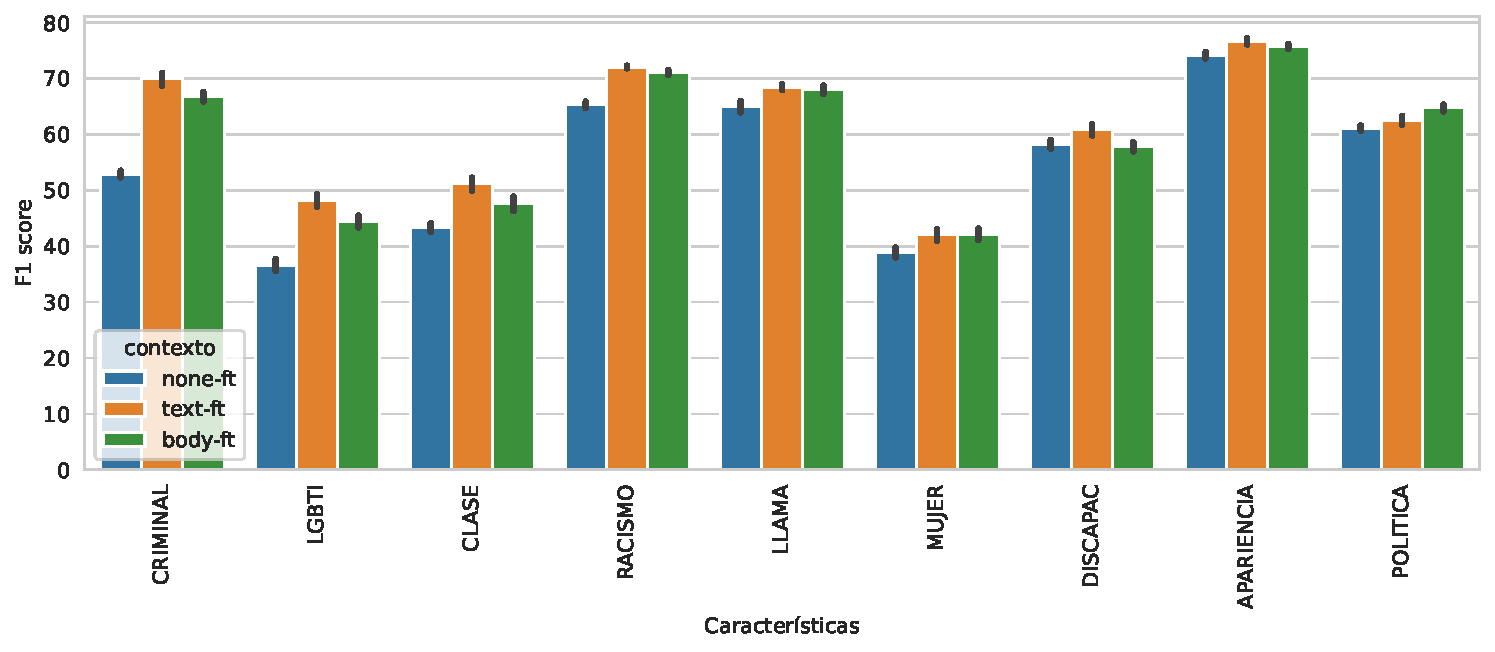
\includegraphics[width=\textwidth]{img/06/task_b_scores.pdf}
    \caption{Métrica F1 para cada característica de la tarea granular, ordenadas de mayor a menor de acuerdo a la diferencia entre el modelo sin contexto y el modelo contextualizado. }
    \label{fig:barplot_task_b_results}
\end{figure*}

La Figura \ref{fig:barplot_task_b_results} muestra los resultados por característica ordenados de mayor a menor según la diferencia de rendimiento entre los clasificadores ajustados a dominio que consumen contexto y aquellos que no lo hacen. Para todas las características se observa una mejora estadísticamente significativa al correr un test Mann-Whitney U ($p \leq 0.005$, p valores ajustados por múltiples comparaciones con Benjamini-Hochberg \cite{benjamini1995controlling}). Las diferencias más sustanciales se dan en el caso de CRIMINAL ($+17$ puntos F1 de diferencia), LGBTI ($+12$ puntos), CLASE ($+8$ puntos), y RACISMO (casi $+7$). Del otro lado, las características con menos mejora son APARIENCIA y POLITICA, algo esperable dado que el fenómeno tiene características poco dependientes del contexto como observamos en algunos ejemplos de la Sección \ref{sec:analisis_dataset_por_caracteristica} y por la misma definición y ejemplos considerados (ver Apéndice \ref{app:05}). Finalmente, y como resumen de estas tablas, se observa que los modelos con contexto simple son los que mejor performance tienen, en general y para cada característica, con la excepción de POLITICA.


\begin{figure}[t]
    \centering
    \small
    % \begin{subfigure}[b]{0.5\textwidth}
    %     \centering
    %     \caption{Precisión}
    %     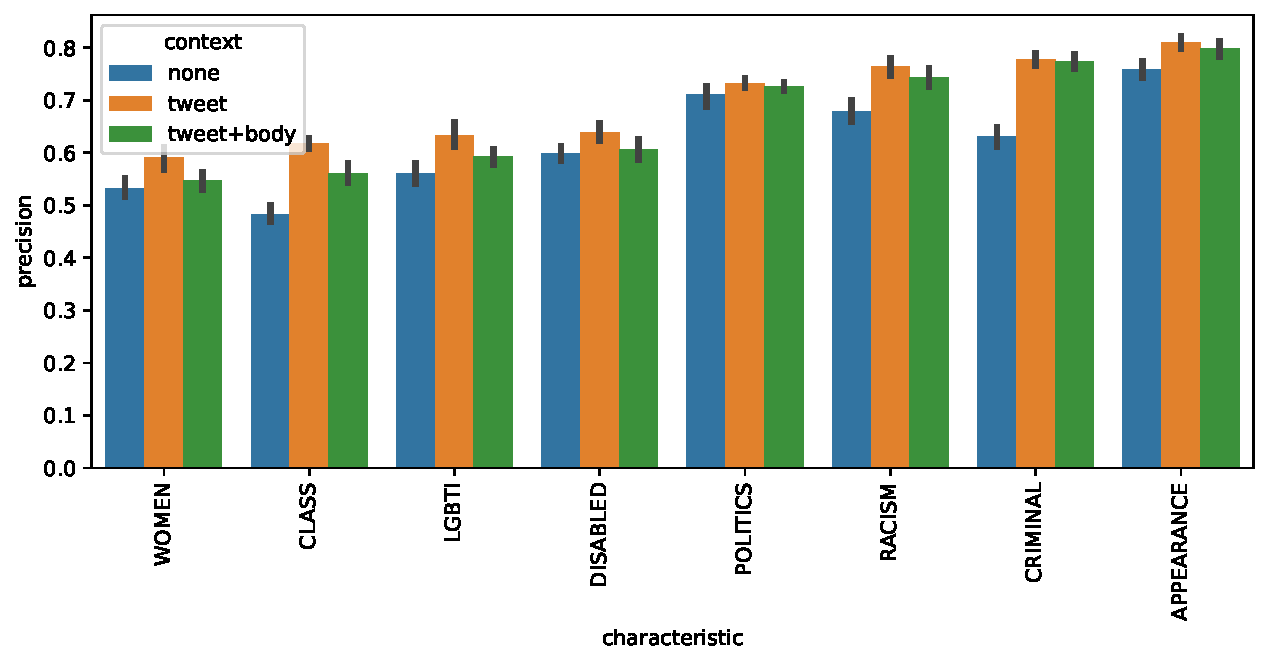
\includegraphics[width=0.99\textwidth]{img/06/precision_barplot.pdf}
    % \end{subfigure}
    \begin{subfigure}[b]{0.45\textwidth}
        \centering
        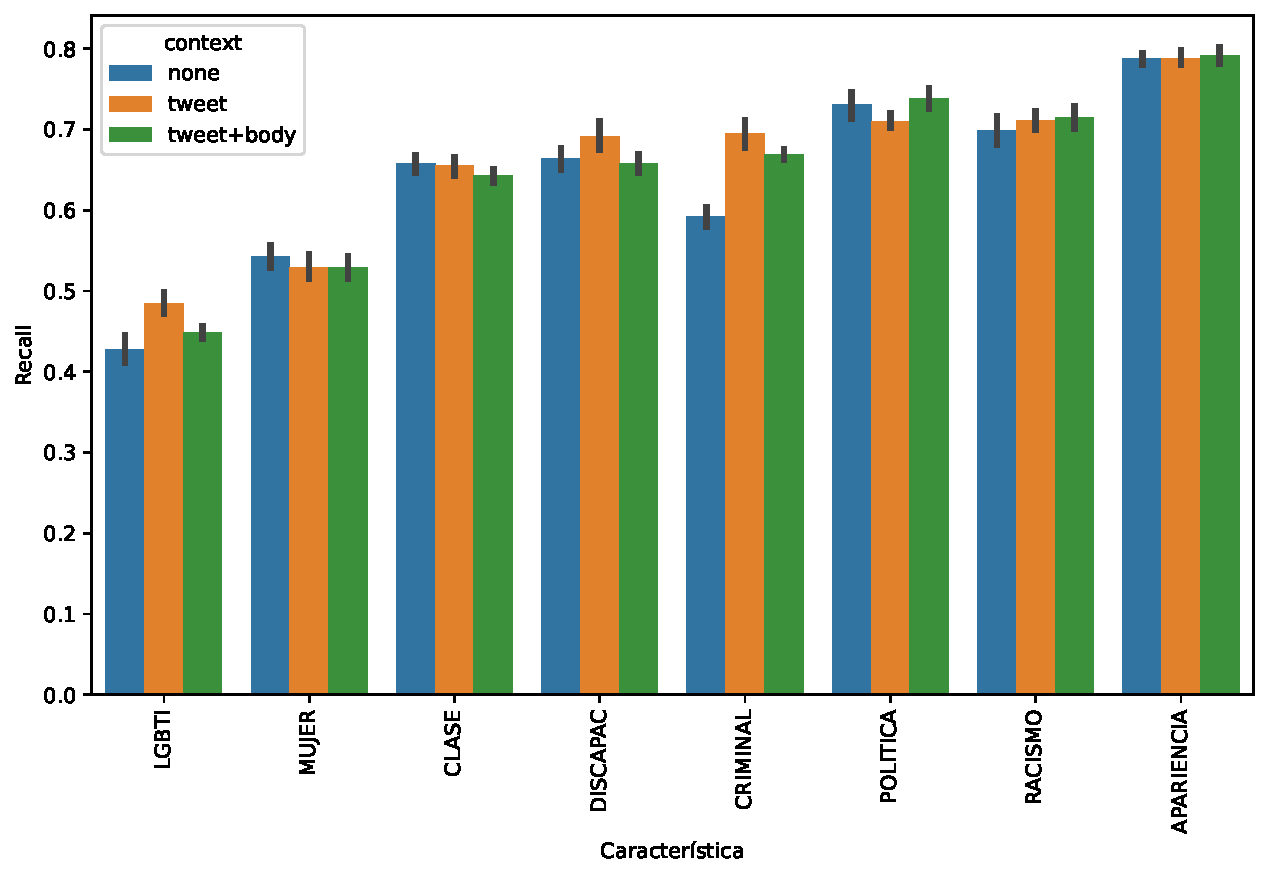
\includegraphics[width=\textwidth]{img/06/exact_recall_barplot.pdf}
        \caption{Sensibilidad exacta}
        \label{subfig:exact_recall}
    \end{subfigure}
    \begin{subfigure}[b]{0.45\textwidth}
        \centering
        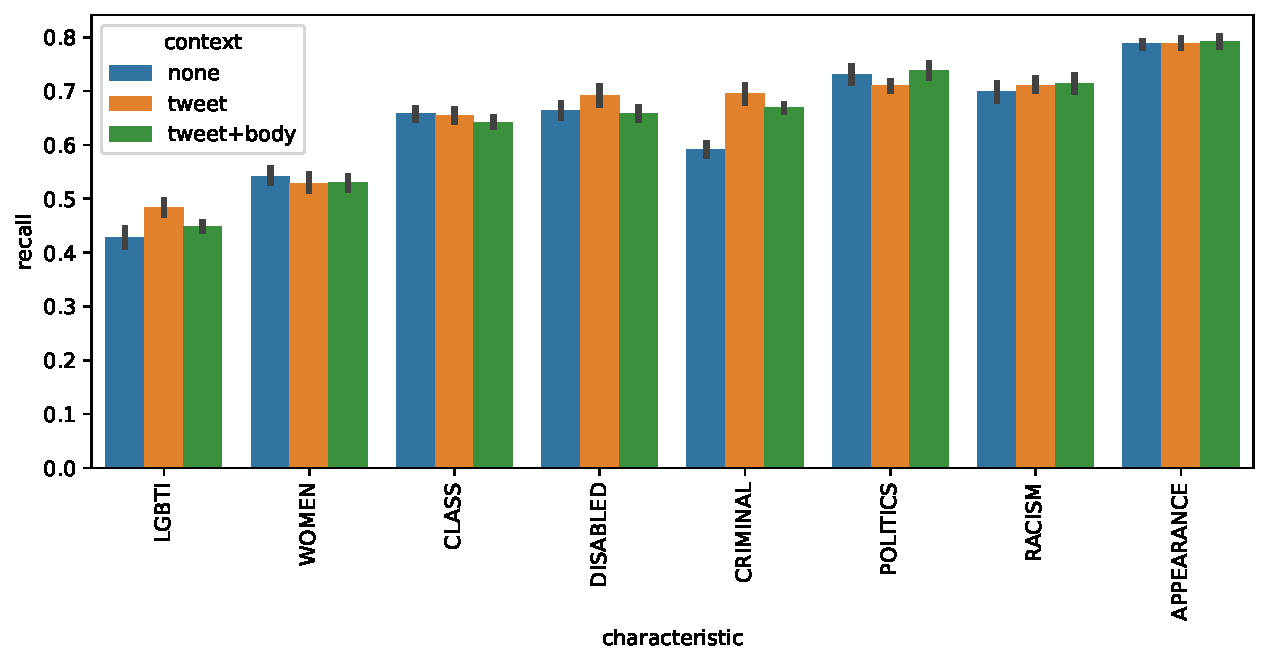
\includegraphics[width=\textwidth]{img/06/hate_recall_barplot.pdf}
        \caption{Sensibilidad total}
        \label{subfig:total_recall}
    \end{subfigure}
    \caption{Precisión y sensibilidad para cada característica de la tarea granular. Las diferentes barras marcan el tipo de contexto que recibe el clasificador. Sensibilidad exacta (Figura \ref{subfig:exact_recall}) cuenta la sensibilidad sobre la salida exacta de cada categoría, mientras que la sensibilidad total cuenta como recuperado un tweet si al menos alguna característica del clasificador lo marca como discurso de odio.}
    \label{fig:precision_recall_granular_classifier}
\end{figure}

Una forma distinta de evaluar el rendimiento de los clasificadores granulares es de acuerdo a su sensibilidad o capacidad de recuperación de comentarios discriminatorios, aún cuando esto ocurra por el motivo incorrecto. La Figura \ref{fig:precision_recall_granular_classifier} ilustra esta comparación analizando la sensibilidad de dos maneras: exacta, donde consideramos recuperado un tweet sólo si el clasificador acierta a la característica analizada (es decir, si la característica es MUJER, el clasificador debe predecir MUJER); y total, donde consideramos un tweet recuperado si alguna característica es marcada por el clasificador independientemente de si es la correcta. Podemos ver que la categoría MUJER pasa de ser la de menor sensibilidad a dejar a la categoría LGBTI como la que tiene menor tasa de comentarios ofensivos recuperados. Análogamente, la categoría CLASE obtiene una mejora sustancial en su sensibilidad, algo compatible con el hecho de su solapamiento con otras características como RACISMO, POLITICA y CRIMINAL observado en la Figura \ref{fig:heatmap_characteristics}. También puede observarse que, en líneas generales, el contexto favorece una mejora de la precisión para cada característica y también un mayor recall exacto. Para el caso de la sensibilidad total, el desempeño de los clasificadores se empareja entre las versiones contextualizadas y no contextualizadas para cada característica con la excepción notoria de LGBTI y CRIMINAL.

\begin{table}[hb!]
    \centering
    \begin{tabular}{l P{0.10\textwidth}P{0.10\textwidth} P{0.10\textwidth}P{0.10\textwidth}  P{0.10\textwidth}P{0.10\textwidth}}
                  &\mc{2}{Sin Contexto}& \mc{2}{Tweet}          &  \mc{2}{Tweet + Cuerpo}    \\
                  & Bin   &    Gran         & Bin   &    Gran     & Bin  &   Gran     \\
        \hline
        Precision &  $71.8$ &  $71.1$       &  $74.8$& $\mbf{75.9}$ & $72.8$ & $74.0$ \\
        Recall    &  $60.2$ &  $63.6$       &  $65.3$& $\mbf{66.7}$ & $64.1$ & $66.0$ \\
        F1        &  $65.5$ &  $67.1$       &  $69.7$& $\mbf{71.0}$ & $68.1$ & $69.7$ \\
        Macro F1  &  $79.8$ &  $80.6$       &  $82.2$& $\mbf{83.0}$ & $81.3$ & $82.2$ \\
        \hline
        \end{tabular}
    \caption{Desempeño de los modelos para la tarea de detección binaria de discurso de odio. Los modelos considerados son modelos \beto{} ajustados a dominio que consumen tres tipos de entrada: sin contexto, tweet, y tweet+cuerpo. Dos posibles entrenamientos fueron evaluados: sobre la tarea binaria (\tbf{Bin}) o sobre la tarea granular (\tbf{Gran}).}
    \label{tab:plain_vs_granular_hate_detection}
\end{table}


Como se mencionó en la Sección \ref{sec:tasks}, un clasificador sobre la tarea granular puede convertirse fácilmente en uno para la tarea binaria tomando la disyunción lógica de sus salidas: si se detecta al menos una característica ofendida, entonces el tweet contiene discurso de odio. De esta forma, podemos evaluar el desempeño en la tarea binaria de aquellos clasificadores entrenados para la tarea granular. La Tabla \ref{tab:plain_vs_granular_hate_detection} muestra esta comparativa para las distintas métricas sobre los clasificadores ajustados a dominio. Podemos observar que, en todos los casos, entrenar el modelo sobre la tarea granular produce pequeñas mejoras en la performance de los clasificadores entrenados sobre la tarea binaria (aproximadamente $+0.8$ puntos de Macro F1 en cada de uno).



\section{Análisis de error}

En esta sección realizamos un análisis de los errores de los clasificadores y comparamos sus distintas variantes. Para ello, analizamos las diferencias entre:

\begin{itemize}
    \item las predicciones del mejor clasificador en términos de performance contra las etiquetas doradas del dataset.
    \item las predicciones del mejor clasificador contextualizado contra las predicciones del mejor clasificador no contextualizado.
    \item las predicciones entre los clasificadores entrenados sobre contra las predicciones de los entrenados sobre la tarea binaria.
\end{itemize}

Para analizar los errores de los modelos, elegimos el clasificador de mejor performance sobre la tarea granular: el clasificador que consume el contexto más el tweet de la noticia, entrenado sobre un \beto{} ajustado a dominio (ver Tabla \ref{tab:task_b_results}). De una manera similar a lo que realizamos en la Sección \ref{sec:hateval_error_analysis}, entrenamos diez clasificadores y analizamos el error sobre el ensamble de voto mayoritario. Para ver los casos más problemáticos, analizamos aquellas características donde peor desempeño muestran los clasificadores: MUJER, LGBTI, y CLASE. Por lo observado en la Figura \ref{fig:precision_recall_granular_classifier}, los clasificadores tienen una sensibilidad muy baja para estas tres características, por lo cual centraremos nuestro análisis en los casos falsos negativos.


\begin{table}[t]
    \centering
    \small
    \begin{tabular}{p{0.03\textwidth} p{0.45\textwidth} p{0.40\textwidth}}
          &Contexto & Comentario \\
        \hline
        1 & Contó que era lesbiana, su papá le confesó que era gay y ahora su madre se enamoró de una mujer, lo que inspiró su segundo film & WTF. Mucho ESI los degeneró... \\
        \rule{0pt}{3ex}2 &                        & @usuario Esta familia tiene los genes alterados \\
        \hline
        3 & Oscar González Oro ya está instalado en el Uruguay: "Recuperé mi libertad" & Ahora quedate allá, y hablá mal d Macri d nuevo pa tener rating. Y opiná q los taxi boy uruguayos son mas educados q los escorts argentinos! Ano abierto! \\
        \hline
        4 & ¿Por qué un beso entre dos hombres los vuelve tan violentos?": la vida después de haber sido víctima de ataques  homofóbicos &  Será xq va contra la naturaleza de la raza... \\
        \hline
        5 & ``¿Por qué no vemos médicos trans?'': el reclamo de un prestigioso cardiólogo para que América sea más inclusiva & Es difícil ser médico con la cabeza quemada \\
        \rule{0pt}{3ex}6  &  & porque un enfermo no cura a otro enfermo \\
        \hline
        7 & ``Te amo''. La emotiva dedicatoria de Luis Novaresio a su pareja en su cumpleaños & \emoji{face-vomiting}\emoji{face-vomiting}\emoji{face-vomiting} \\
        \hline
        8 & Elizabeth Gómez Alcorta: ``Por la pandemia, vamos a tener una suba de los femicidios y travesticidios'' &  Travesticidios... Osea asesinatos de tipos con peluca y tetas \\
        \hline
        9 & Mariana Genesio Peña pasa su cuarentena total con guantes, barbijo y desnuda: ``Mi cuerpo es el planeta Tierra'' & Coronavirus nivel pelotudo en bolas	\\
        \rule{0pt}{3ex}10 &    & Con 3 piernas cualquiera es feliz!!!	\\
        \rule{0pt}{3ex}11 &    & pasa la cuarentena rascándose las bolas \\
        \hline
        12 & Tras una ráfaga de más de 20 disparos asesinaron a una mujer trans en Rosario & Cómo no saco su escopeta y aplicó la defensa propia?! \\
        \rule{0pt}{3ex}13 & & @usuario Salió de caño... cuac!	\\
        \hline
    \end{tabular}
    \caption{Falsos negativos para la característica LGBTI. Ninguno de los diez clasificadores que consumen contexto y texto indentificaron como discriminatorios a estos comentarios. }
    \label{tab:lgbti_error_analysis}
\end{table}



La Tabla \ref{tab:lgbti_error_analysis} muestra una selección de comentarios discriminatorios para la característica LGBTI que no son detectados por los clasificadores. De estas instancias, y observando también aquellos casos donde sí puede detectar el discurso discriminatorio de esta categoría, podemos esbozar algunas posibles razones detrás de estos errores. En primer lugar, ciertos mensajes altamente ofensivos son complejos de entender: por ejemplo, los que tratan de ``enfermos'' o mencionan cuestiones de la genitalidad (ejemplos 5 y 6). Estas ofensas son realizadas por los usuarios de maneras tan sofisticadas que difícilmente un modelo de lenguaje pueda entender, como metáforas varias que hacen referencia a la genitalidad de una mujer trans (ejemplos 10 y 12) o bien refiriéndose al objetivo de la ofensa con un género distinto al autopercibido (ejemplos 8 y 9),

Algunos comentarios y sus contextos --como los ejemplos 3, 7, 9, 10 y 11-- omiten información acerca de la sexualidad o género sobre quienes versa la noticia. Esta información faltante no permite a los clasificadores (ni tampoco a un humano que carezca de esta información) entender completamente el caracter discriminatorio de los mensajes.


\begin{table}[t]
    \centering
    \small
    \begin{tabular}{p{0.03\textwidth} p{0.40\textwidth} p{0.40\textwidth}}
        & Contexto & Comentario \\
        \hline
        1 & Martha Rosenberg: ``En situación de pandemia, legalizar el aborto es más urgente que nunca'' & Quien es esta vieja?. No debería estar tejiendo? \\
        \hline
        2& Mara Gómez: la historia de la primera futbolista trans en el torneo argentino  &  Feminismo pierde de nuevo... ya le metieron un tipo... jaja punto para el patriarcado...	 \\
        \hline
        3& Tras una ráfaga de más de 20 disparos asesinaron a una mujer trans en Rosario & Las feministas en modo error 404 al no saber si celebrar o ofenderse  \\
        \hline
        4& El desesperado pedido de Actrices Argentinas ante la violencia de género en cuarentena: ``Es urgente'' & Que risa me dan las feministas!!! Ignorantes.	 \\
        \hline
        5& Leche de cucaracha, la nueva bebida nutritiva: ¿quién se anima a probarla? & No me digas q la hija de CFK está embarazada y ya sale leche por esos senos	 \\
        \hline
        6& Los fans de Florencia Kirchner le piden casamiento por Instagram & Zoofilia \\
        \rule{0pt}{3ex}7&                       & Hdp tienen que tener estomago para querer casarse con terrible adefesio \\
        \hline
        8& Rosario: para sacar una licencia de conducir habrá que hacer un curso de perspectiva de género & Te quieren adoctrinar desde cualquier ámbito, y se están metiendo en todo para que empieces a hablar como el orto, como a ellas les gusta.	\\
        \rule{0pt}{3ex}9&   & El que choca más feministas le dan más años de licencia	\\
        \hline
        10& Por qué los países liderados por mujeres parecen haber respondido mejor a la crisis del coronavirus & Son mujeres inteligentes que se dejan asesorar de sus esposos \\
        \hline
        11& Joe Biden presentó su nuevo equipo de comunicación compuesto enteramente por mujeres & Será equipe conche seque?	\\
         \hline
    \end{tabular}
    \caption{Falsos negativos para la característica MUJER. Ninguno de los diez clasificadores que consumen contexto y texto (ajustados a dominio) lograron identificar como discriminatorios a estos comentarios para ninguna otra característica. }
    \label{tab:women_error_analysis}
\end{table}




En el caso de MUJER, restringimos nuestro análisis a aquellos ejemplos que no son detectados por otras características ya que, por lo observado en la Figura \ref{fig:precision_recall_granular_classifier}, muchos ejemplos están en la frontera de otras categorías y son detectados por ellas. La Tabla \ref{tab:women_error_analysis} muestra una selección de estos falsos negativos, donde podemos apreciar que algunos ejemplos están en el borde borde de ser simplemente ofensivos (ejemplo 1 y posiblemente 6 y 7) o contienen mensajes irónicos complejos de descifrar (ejemplo 3, que las feministas celebren por la muerte de una mujer trans, o ejemplo 9, hablar de chocar mujeres en un curso de manejo). Esto es esperable dado el acuerdo relativamente bajo para la categoría MUJER en el etiquetado de este dataset reportado en la Tabla \ref{tab:dataset_figures}.




\begin{table}[ht!]
    \centering
    \footnotesize
    \tbf{CRIMINAL}
    \begin{tabular}{p{0.03\textwidth} p{0.04\textwidth} p{0.40\textwidth} p{0.40\textwidth}}
        \hline
        & Tipo & Contexto & Comentario \\
        \hline
         1 & \multirow{2}{*}{FN} &Una policía baleó y mató a un joven de 17 años que la atacó con una tijera en Moreno url	& \emoji{clapping-hands} excelente!  \\
                             %&                                                                                          &  bellezaa \\
        \rule{0pt}{3ex}2 &                &El polémico cortejo del ladrón asesinado por el jubilado en Quilmes                       & Le hubieran puesto una bomba al cortejo \\
         \hline
         \rule{0pt}{3ex}3 & \mr{2}{FP}          & Ivana Nadal se cansó de la criticaran y sorprendió con su respuesta: "Gracias a Dios a fin de año me voy del país" & Esa si es una buena noticia. \\
                             %& Mora Godoy cierra su escuela de tango y remata su vestuario para "poder seguir adelante" & Adoro los finales felices \\
         \rule{0pt}{3ex}4 &                &¿Se va del país? Juana Viale estaría tramitando la ciudadanía uruguaya & Q bueno ? Una mierda menos . Q se quede alla \\
         \hline
    \end{tabular}
    \rule{0pt}{3ex}\tbf{LGBTI}
    \begin{tabular}{p{0.03\textwidth} p{0.05\textwidth} p{0.45\textwidth} p{0.40\textwidth}}
        \hline
        \rule{0pt}{3ex}6 & \mr{2}{FN} & ``Te amo''. La emotiva dedicatoria de Luis Novaresio a su pareja en su cumpleaños & Definitivamente no acepto esta degeneración repugnante de la humanidad. \\
        \rule{0pt}{3ex}7 &        &  Mara Gómez: la historia de la primera futbolista trans en el torneo argentino & Sigue siendo HOMBRE, que por GENÉTICA, no por una ideología u orientacion sexual, GE-NÉ-TI-CA, es más fuerte que la mujer. \\

                    %&  Contó que era lesbiana, su papá le confesó que era gay y ahora su madre se enamoró de una mujer, lo que inspiró su segundo film& Revisen esa casa, los están envenenando\\
        \hline
        \rule{0pt}{3ex}8  & \mr{2}{FP} &  URGENTE: Un hombre se incrustó con su auto en la puerta de la Embajada de China y aseguró que tenía explosivos & No es hombre . Es un boludo	\\
         \rule{0pt}{3ex}9   &      &  Detuvieron al hombre que admitió violar a su hija en audios de WhatsApp y fue tendencia en redes: un tío lo entregó & Degenerado \emoji{face-vomiting} \\
        \hline
    \end{tabular}
    \rule{0pt}{3ex}\tbf{CLASE o RACISMO}
    \begin{tabular}{p{0.03\textwidth} p{0.05\textwidth} p{0.45\textwidth} p{0.40\textwidth}}
        \hline
        10 & \mr{3}{FN} & Las organizaciones sociales salieron al cruce de la acusación de Sergio Berni por la toma de tierras:  ``La falta de vivienda no se resuelve con balas'' & Si, los podemos cagar matando a todos y listo \\
                   %&                                       & @usuario Dale alas y planes a los cuervos y veras cómo te sacan los ojos  \\
        \rule{0pt}{3ex}11 & & La temporada de verano en la Costa Atlántica empezó con un corte total en la Ruta 2: organizaciones sociales piden canastas navideñas & Hay que desparasitar urgente el país. \\
        \rule{0pt}{3ex}12 & &  La pregunta billonaria: ¿China debería pagar el costo de la pandemia? & Si obviamente y desaparecer de la faz de la tierra. Mira el quilombo que armó. Se nos están muriendo todos... \\
        \hline
        13 & \mr{4}{FP} & Javier Milei confirmó que va ``a militar en política'' junto a José Luis Espert para que ``en 35 años la Argentina sea primera potencia mundial'' & Otro parásito	 \\
                   %& Leche de cucaracha, la nueva bebida nutritiva: ¿quién se anima a probarla? & Uds pueden producir litros, son todes cucarachas y ratas!!!  \\
                   \rule{0pt}{3ex}14 &            & Martha Rosenberg: ``En situación de pandemia, legalizar el aborto es más urgente que nunca'' & La verdad que sí...así se dejan de reproducir!!!  \\
                   \hline
        \hline
    \end{tabular}
    \caption{Ejemplos donde el clasificador contextualizado acierta y el no contextualizado falla. FN marca que el clasificador no contextualizado no detecta el comentario como discriminatorio (ni para la característica marcada ni para otras) mientras que el contextualizado sí lo hace; FP es al revés, que el clasificador no contextualizado marca erróneamente el comentario como discriminatorio  }
    \label{tab:context_vs_no_context_error}
\end{table}


En la Tabla \ref{tab:context_vs_no_context_error} podemos observar una selección de ejemplos donde el clasificador contextualizado acierta en su predicción mientras que el modelo sin contexto se equivoca, separados en falsos negativos (el modelo no contextualizado no logra detectarlos) y falsos positivos (el modelo no contextualizado predice equivocadamente que son discriminatorios). En el caso de LGBTI, la información contextual permite desambiguar casos como los 7 y 8, muy similares pero con un contexto sumamente distinto. Un problema que se puede apreciar es que el clasificador no contextualizado --al ser entrenado con datos etiquetados de manera contextualizada-- aprende correlaciones espurias como que las celebraciones son discriminatorias (ejemplo 16).

La comparativa entre los clasificadores entrenados sobre la tarea binaria y la tarea granular es más difícil de interpretar. Si bien se observa que entre los falsos negativos del clasificador binario se encuentra una proporción más alta de tweets racistas, es difícil elucidar una razón detrás de esto. En la Tabla \ref{tab:fine_vs_plain_comparison} del Apéndice \ref{app:06} se encuentra una muestra de ejemplos en los cuales el clasificador granular acertó y el binario falló.




\section{Discusión}

Para analizar el impacto del contexto en la detección de discurso de odio, planteamos dos tareas de clasificación sobre el dataset construído en el capítulo \ref{chap:05_dataset_creation}: la tarea de detección binaria, donde respondemos si un comentario contiene discurso de odio; y una tarea de detección granular, donde se debe mencionar la o las características protegidas ofendidas (si agrede a las mujeres, al colectivo LGBTI, si es racista, etc). En ambas tareas planteadas propusimos clasificadores que consumen 3 tipos de entrada: el comentario sin contexto, el comentario con el contexto del tweet al que responden, y el comentario más el tweet al que responde y también el texto del artículo. Pudimos observar que el contexto parece dar una mejora moderada pero significativamente estadística en la tarea de detección del discurso de odio (alrededor de 3 puntos F1), y una mejora considerable en la tarea característica ofendida (alrededor de 6 puntos F1 medios).

Esto, en algún punto, indicaría que el contexto puede ser aprovechado para mejorar los algoritmos de detección de discurso de odio. Si bien este resultado podría estar en aparente contradicción con trabajos recientes que no encontraron ninguna mejora en el uso del contexto en la detección de toxicidad \cite{pavlopoulos2020toxicity}, se puede señalar que la detección del discurso de odio es una de las formas más complejas de comportamiento ``tóxico'' y, como tal, podría permitir que los clasificadores tengan más información para predecir si el texto dado es odioso o no. Otra razón detrás de este resultado es el dominio de nuestro conjunto de datos: mientras que \citet{pavlopoulos2020toxicity} usa el contexto conversacional, nosotros usamos el título y el cuerpo del artículo como contexto para los comentarios de los usuarios. Más recientemente, y como marcamos en la sección de trabajo previo, en \citet{xenos-2021-context} han observado que, restringiendo el análisis a un subconjunto de comentarios sensibles al contexto (ver \ref{sec:06_classification_previous} y \ref{sec:dataset_previous} para más información), la performance de los algoritmos de detección de toxicidad mejoran de manera significativa.

La utilización de un contexto más largo como el artículo de la noticia no mejora la performance de los clasificadores en nuestros experimentos. Hay varias interpretaciones posibles de esto: en primer lugar, los humanos suelen contestar sin leer el artículo, con lo cual este resultado pareciera ser coherente con esta observación. Por otro lado, los humanos solemos tener acceso a un contexto mucho más rico, muchas veces equivalente a haber leído la nota, algo que nuestros clasificadores carecerían. Podría también esto ser atribuido al modelo pre-entrenado que usamos para codificar esto (BETO, la variante en español de BERT) suele estar pre-entrenada para textos más cortos. Teniendo esto en cuenta, realizamos el ajuste de dominio usando el contexto largo, pero aún así el desempeño del clasificador que consume este contexto largo se mantuvo por debajo del que usaba el contexto simple.

El análisis del error realizado demostró que, si bien el contexto pareciera mejorar la detección de discurso de odio, para muchas características protegidas se mantiene aún como una tarea difícil. Un caso ejemplificador de esto es la discriminación contra el colectivo LGBTI. En las instancias del dataset --y en muchos de los ejemplos en los que el algoritmo de detección falla--  puede verse que las agresiones contra este colectivo y sus miembros son sumamente sofisticadas, lejos de las agresiones meramente basadas en insultos u otras palabras ofensivas. Nuestros clasificadores, aún en sus mejores versiones (usando ajuste de dominio y contexto) obtuvieron una baja performance en la detección de este fenómeno (alrededor de $0.5$ F1 score) dando cuenta que es un problema no trivial y merece ser analizado más detenidamente debido a la complejidad de estos mensajes, que suelen reunir ironía, metáforas, y otros artilugios que hacen difícil su detección.

En el caso de la categoría mujer, inesperadamente, también obtuvimos una performance muy baja en la detección de agresiones misóginas. En el análisis de error, podemos observar que tenemos casos complejos de descifrar que fueron marcados por nuestros anotadores: por ejemplo, ataques velados a mujeres víctimas de violación (llamarlas mentirosas). \todo{Escribir un poco más sobre esto}

Algo que debe ser tenido en cuenta para matizar estos resultados es que utilizamos un amplio espectro de características protegidas. Incluso, la que más se beneficia del contexto es una que introdujimos ad-hoc para este experimento (discurso de odio contra criminales). En contrapeso, otras características ``no convencionales'' son poco beneficiadas por el contexto (como discurso de odio en base a la apariencia, opinión política y discapacidad).

Un resultado que también observamos es que pareciera ser que nuestros clasificadores mejoran leve pero significativamente su performance en un contexto de aprender cada característica por separado en vez de sólo aprender a distinguir la etiqueta binaria de discurso de odio. Si bien la mejora es marginal (cerca de un punto de F1) y no es observable de manera subjetiva mediante un análisis de error, una posible razón detrás de esto es que la señal más precisa acerca de la categoría ofendida puede ayudar a distinguir mejor las fronteras de este fenómeno. Aún cuando esta mejora no fuese tal, poder tener una salida más interpretable y granular es mejor que simplemente obtener una predicción binaria.

Una limitación importante de este estudio es que el entrenamiento lo realizamos sobre datos entrenados únicamente observando el contexto. Entrenar a los clasificadores no contextualizados sobre estas etiquetas induce a los clasificadores a tomar decisiones erróneas, como asumir que celebraciones son discurso de odio debido a instancias que --con contexto-- tienen esa naturaleza. Un estudio más completo del impacto del contexto en esta tarea debería incluir los datos entrenados sin contexto.

En el terreno de la aplicación, un problema práctico de este resultado es que no siempre tenemos un contexto disponible para un texto dado. Incluso si podemos encontrarlo, a veces este contexto puede no ser en forma de artículo de noticias, sino como un hilo de conversación o incluso de alguna otra representación. Teniendo en cuenta alguna de las consideraciones hechas en esta discusión, una posible línea de investigación seria la de incorporar distintos tipos de contexto, desde más mensajes en el hilo de la conversación, conocimiento estructurado (por ejemplo, la propuesta en \emph{ERNIE} \cite{zhang2019ernie} o \emph{KI-BERT} \cite{faldu2021ki}) o bien una combinación de diversas fuentes, incluso multimodales.

\section{Conclusiones}

En este capítulo hemos realizado experimentos de clasificación sobre el dataset construído en el capítulo anterior, focalizándonos en analizar el impacto de la utilización del contexto en la performance de los modelos. Planteamos dos tareas: una tarea binaria --detectar si existe discurso de odio o no-- y una tarea granular --definir qué categorías son atacadas en un tweet, si es que las hay--. Para ambas tareas, los modelos contextualizados obtienen mejoras significativas en la performance, dando indicios de que información adicional al comentario analizado puede ayudar a detectar el discurso de odio. Si bien en nuestros experimentos el contexto más pequeño (el tweet del artículo de la noticia) fue el que mejor resultados obtuvo, una línea de trabajo futuro podría explorar otras formas de incorporar el contexto más largo -- en este caso, el artículo de la noticia.

Así mismo, observamos una pequeña pero estadísticamente significativa mejora en la detección de discurso de odio al entrenar un clasificador granular al ser evaluado de manera binaria. En este caso, obtenemos una ventaja al obtener una salida más interpretable de las características ofendidas, y que además que no sólo no empeora la performance de nuestro clasificador sino que hasta incluso mejora levemente.

Del análisis de error, se observa que algunas categorías del discurso de odio se muestran elusivas para los algoritmos de detección. Uno de estos casos son los mensajes abusivos contra la comunidad LGBTI+, conteniendo mensajes semánticamente complejos, implícitos y con metáforas que son esquivas para los modelos propuestos. A pesar de estas limitaciones, esta característica fue una de las más beneficiadas por la adición de contexto, aunque su desempeño sigue siendo bajo, teniendo una puntuación de F1 de alrededor de 0.5.

Podemos concluir que los datasets de discurso de odio deberían --en la medida de lo posible-- contener \textbf{información contextual} sobre los comentarios analizados. Esta información puede darse en forma de artículos de noticias, como un hilo de conversación, o incluso como otras formas --por ejemplo, como una base de conocimiento. Sobre esto, trabajo futuro debería explorar el impacto de utilizar esta información adicional para integrarla en algoritmos de detección de discurso de odio. La evidencia de estos experimentos --por ahora preliminares, y con las limitaciones marcadas en la discusión-- indica que los modelos del estado del arte pueden utilizar esta información para mejorar la detección de discurso de odio en redes sociales. En segundo lugar, los datasets de discurso de odio deberían incluir \textbf{información granular} acerca de las características atacadas --y no sólo una etiqueta binaria-- ya que por un lado esto mejora la interpretabilidad de los algoritmos de detección, y resultados preliminares de este estudio indicarían que mejoran marginalmente la performance en la detección en general.

Finalmente, un aspecto que introdujimos en este capítulo fue el de adaptar un modelo de lenguaje pre-entrenado a su dominio, siendo en nuestro caso los comentarios sobre notas periodísticas en Twitter. Las mejoras que reportó la utilización de estas técnicas fue significativa, en consonancia con otros trabajos recientes. Pasaremos a continuación a estudiar estas técnicas en el marco más general de la clasificación de textos sociales.